\documentclass[xcolor=table]{beamer}
\usepackage[utf8]{inputenc}
\usepackage[T1]{fontenc} 
\usepackage[english]{babel} 
\usepackage{graphicx}
\usepackage{comment}
\usepackage{graphicx,wrapfig,lipsum}
\usepackage{hyperref}
\usepackage{tcolorbox}
\hypersetup{
    colorlinks=true,
    linkcolor=blue,
    filecolor=magenta,      
    urlcolor=cyan,
}
\setbeamertemplate{footline}[text line]{%
  \parbox{\linewidth}{\vspace*{-8pt}\today\hfill\insertshortauthor\hfill\insertpagenumber}}{}

%%Defining the ``proposition'' environment
\newtheorem{proposition}{Proposition} 

%%Sets the beamer theme "Cuerna"
\usetheme{Cuerna} 

\usecolortheme{default}
%Available color themes: default, bluesimplex, brick, lettuce

%%Insert the logo
\logo{
\includegraphics[width=1.7cm]{plots/logo.jpeg}}

%%Title
\title{TELLIE PCA\\Automation}

\author{Michal Rigan\\ %Author
          \texttt{mrigan@snolab.ca}} %e-mail
          
\date{\textbf{Report}\\
\today} %Date or event

\institute{University of Sussex} %%Institution

\begin{document}

{
\setbeamertemplate{footline}{} 
\begin{frame}
  \titlepage %Creates the title page
\end{frame}
}

\begin{frame}{Automation - Why}
\begin{itemize}
	\item TELLIE PCA takes a lot of time - both manpower and detector time (<16h data taking, 2 days processing)
	\item the frequency can be tuned so that we are satisfied with the deadtime	
	\item was the plan since TELLIE was designed
	\item other detector aspects are being automated (shifting)
	\item (automation, if done properly, is good)
\end{itemize}
\end{frame}

\begin{frame}{Monitoring}
\begin{itemize}
	\item there won't be a person looking at the data-taking in real time (as was the case for dedicated runs until now)
	\item need a method to monitor the light intensity fired by TELLIE
	\item don't have immediate access to live NHit data in Orca (this is done by Event builder, and then later available on data stream)
	\item have access to PIN readouts - internal TELLIE reading, corresponds to light intensity, already available to Orca
	\item need to know PIN to NHit correlation and stability
\end{itemize}
\end{frame}

\begin{frame}{PIN vs NHit}
\noindent\makebox[\textwidth]{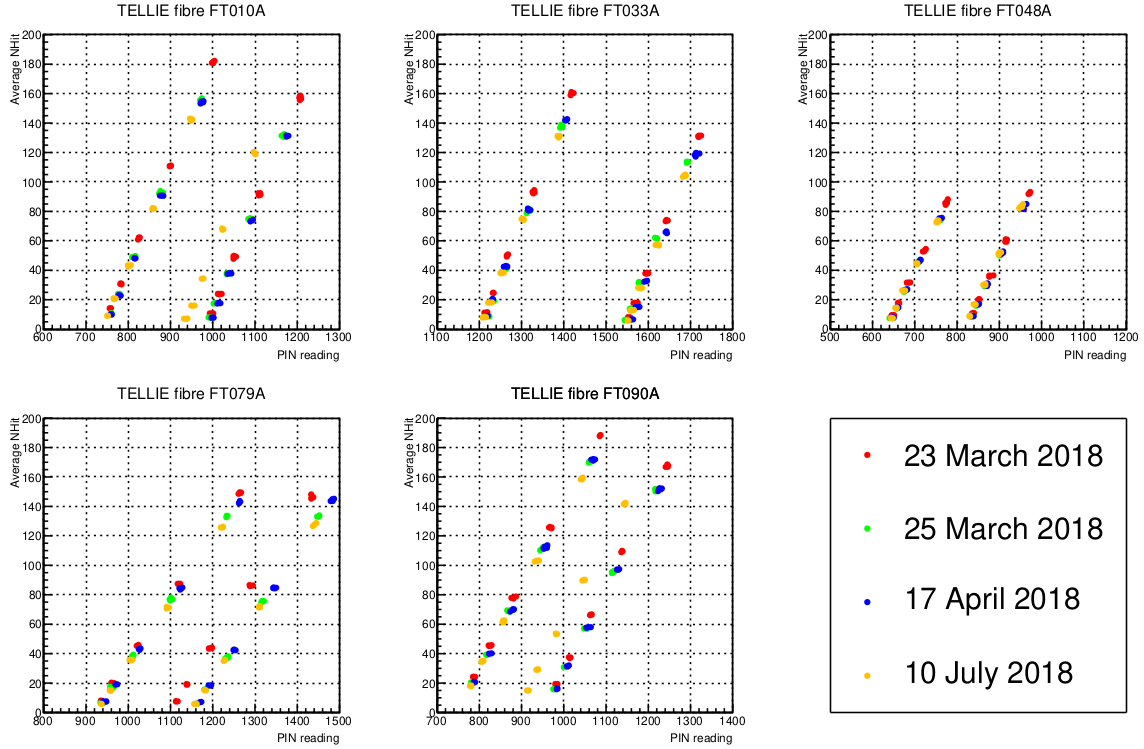
\includegraphics[width=0.85\textwidth]{plots/pin-nhit.png}}
\centering \small reasonably stable over time, only likely to change with changes to detector or TELLIE hw
\end{frame}

\begin{frame}{Automation - How}
\begin{itemize}
	\item data-taking auto
	\item processing + analysis auto
\end{itemize}
\end{frame}

\begin{frame}{Automation: data-taking}
\begin{itemize}
	\item Profiling (less frequently):
	\begin{itemize}
		\item need calibration curves (IPW - PIN)
		\item need tuning curves (PIN - NHit)
	\end{itemize}
	\item need to decide how we want to take the data:
	\begin{itemize}
		\item automate current dedicated running
		\item continuous running alongside Physics
	\end{itemize}
\end{itemize}
\end{frame}

\begin{frame}{Data-taking: calibration curves}
Calibration curves scan the fibre to obtain the PIN to IPW data (we set the IPW, PIN is our internal intensity check)
\noindent\makebox[\textwidth]{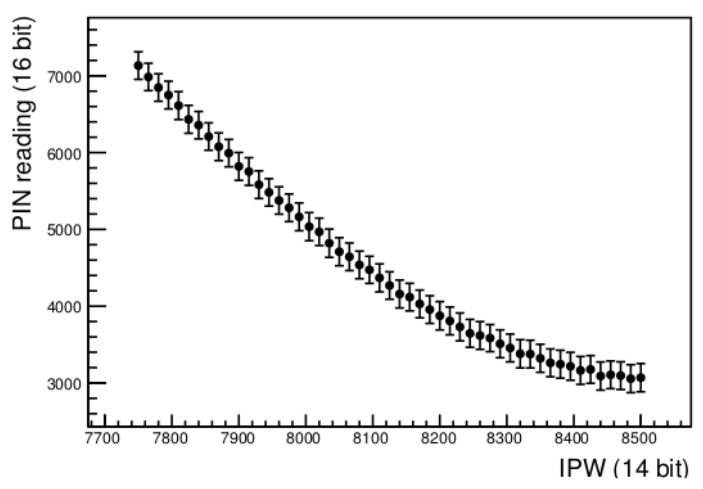
\includegraphics[width=0.85\textwidth]{plots/pin-ipw.png}}
\end{frame}

\begin{frame}{Data-taking: calibration curves}
\begin{itemize}
	\item PIN reading is inversely proportional to the IPW setpoint (this determines the pulse intensity)
	\item up until emission threshold where the PIN becomes flat
	\item LED intensity tends to drift over time with the same IPW, so the PIN readings should be trusted rather than IPW
\end{itemize}
\end{frame}

\begin{frame}{Data-taking: calibration curves}
\noindent\makebox[\textwidth]{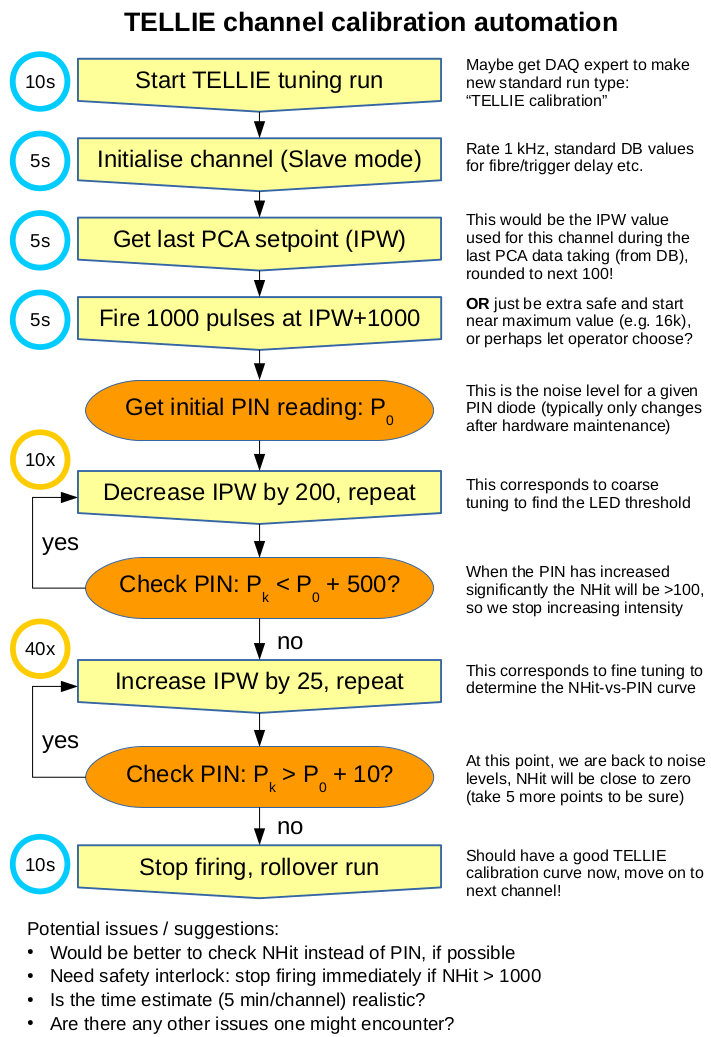
\includegraphics[width=0.435\textwidth]{plots/calib.png}}
\end{frame}

\begin{frame}{Data-taking: tuning curves}
The average EXTA-NHit can be extracted from data by nearline processor, creating PIN-NHit plot. This can be fitted and several parameters can be extracted:
\begin{itemize}
	\item LED emission threshold (lowest IPW producing 0 NHit)
	\item PCA intensity setpoint (IPW corresponding to 45 NHit)
	\item Internal noise level (PIN value below the LED emission threshold)
	\item Fit parameters to match external NHit to PIN reading \\ (y = ax + b)
\end{itemize}
\end{frame}

\begin{frame}{Data-taking: tuning curves}
\noindent\makebox[\textwidth]{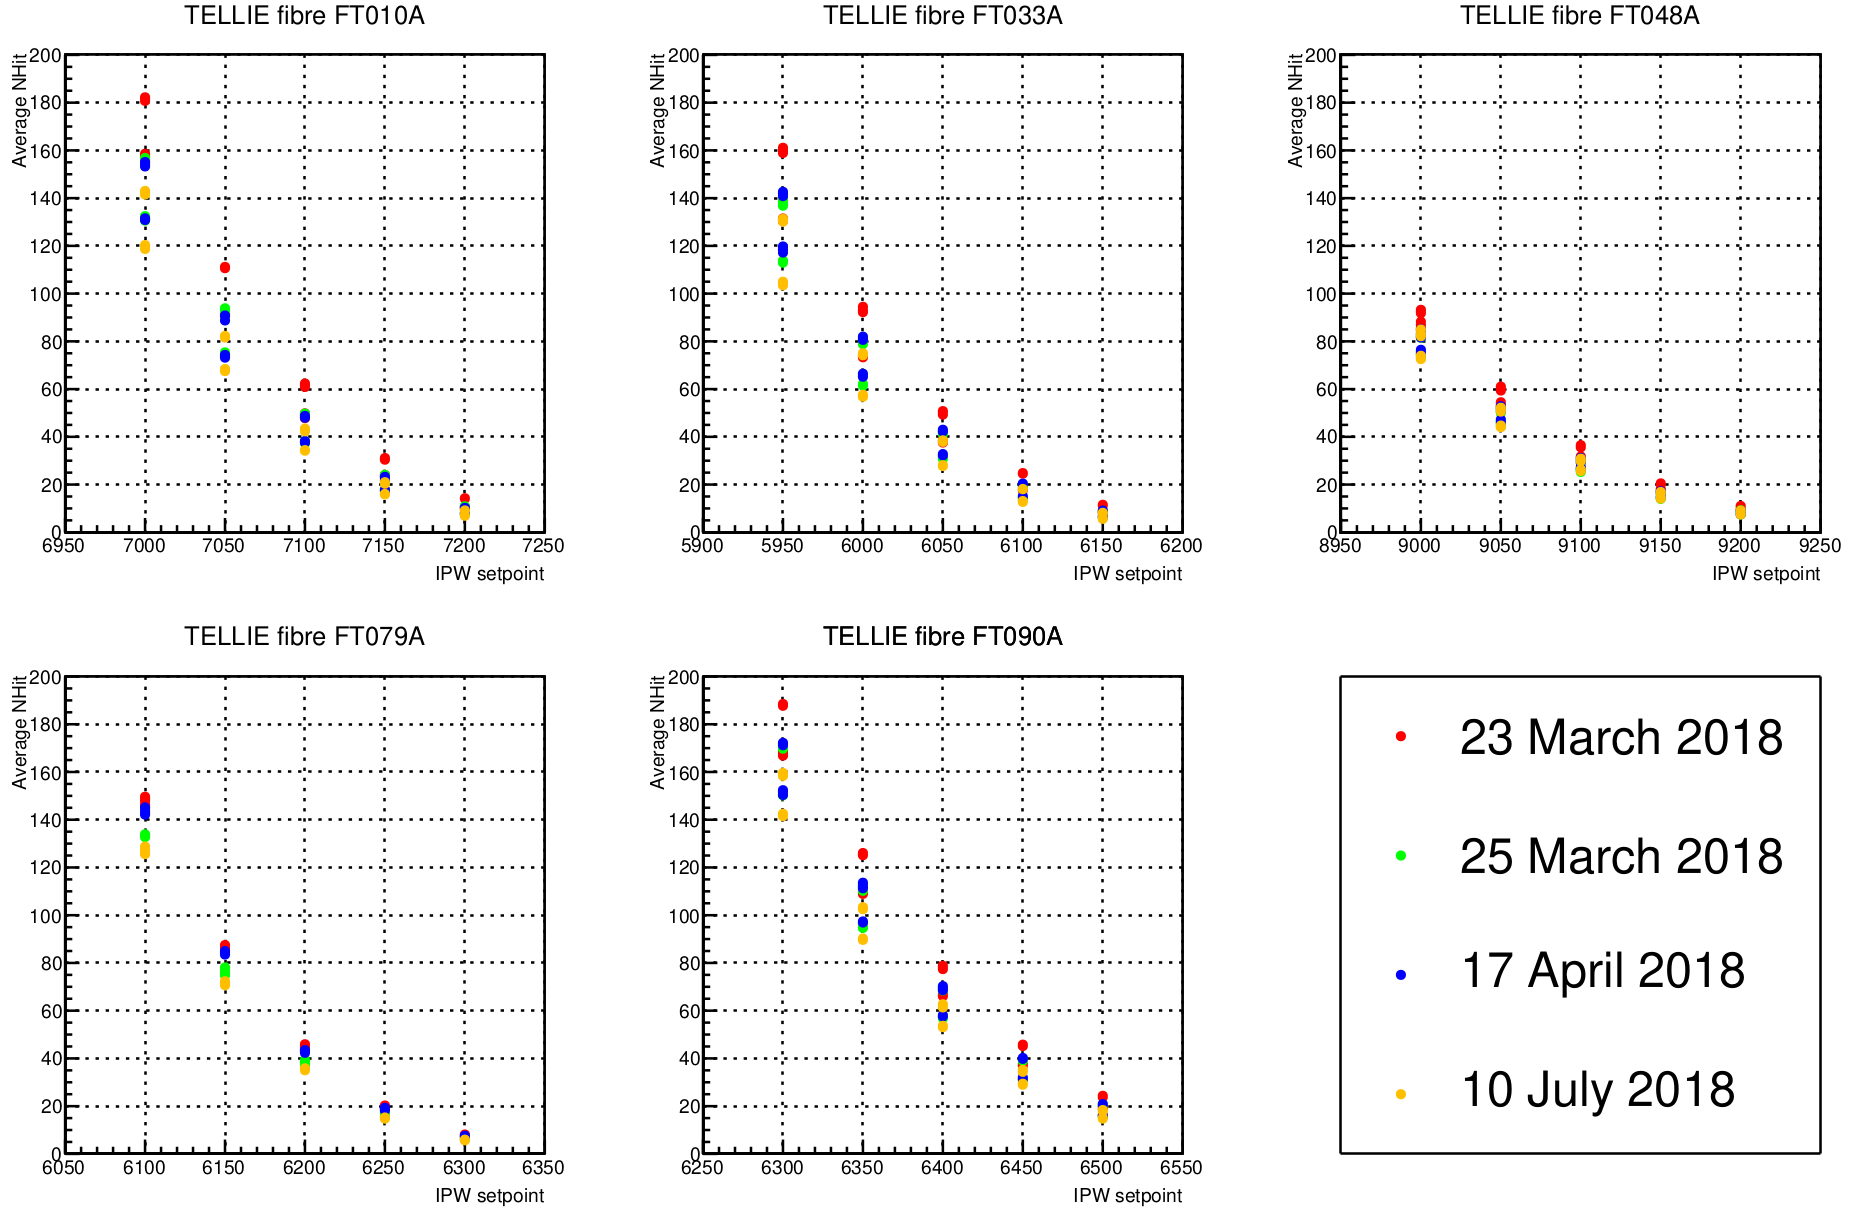
\includegraphics[width=0.95\textwidth]{plots/ipw-nhit.png}}
\end{frame}

\begin{frame}{Data-taking: dedicated}
If we decide to follow the dedicated way = 1 kHz, 200 000 pulses:
\noindent\makebox[\textwidth]{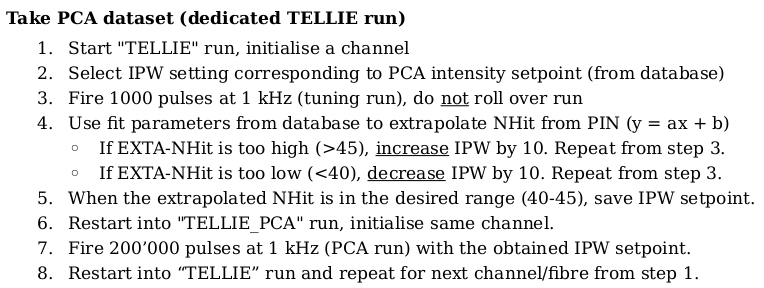
\includegraphics[width=1\textwidth]{plots/dedicated.png}}
\end{frame}

\begin{frame}{Data-taking: dedicated}
\begin{itemize}
	\item this is what is currently done manually by operators
	\item entire dataset = 95 fibres takes 12-16h to complete
	\item automation would greatly facilitate this
\end{itemize}
\end{frame}

\begin{frame}{Data-taking: continuous}
If we decide to follow the continuous method:
\noindent\makebox[\textwidth]{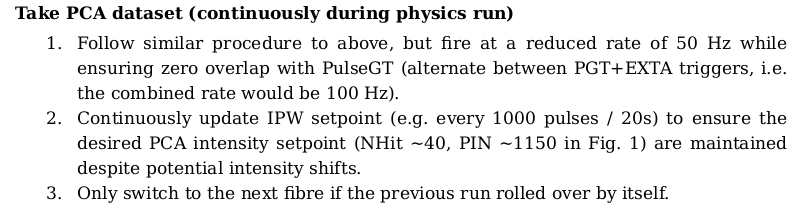
\includegraphics[width=1\textwidth]{plots/continuous.png}}
\end{frame}

\begin{frame}{Data-taking: continuous}
\begin{itemize}
	\item normal physics run would contain 180 000 TELLIE pulses
	\item PulseGT won't steal EXTA triggers (other triggers still can, but the precise timing can be used to flag data)
	\item full PCA set would require 95 completed physics runs ($\sim$ 4 days)
	\item Processing follows when full set is taken
	\item intervention only required when things go wrong
	\item this should increase the detector livetime and reduce need for TELLIE operators
	\item obviously requires a lot of work, and most importantly ORCA knowledge
\end{itemize}
\end{frame}

\begin{frame}{Automation: processing}
\noindent\makebox[\textwidth]{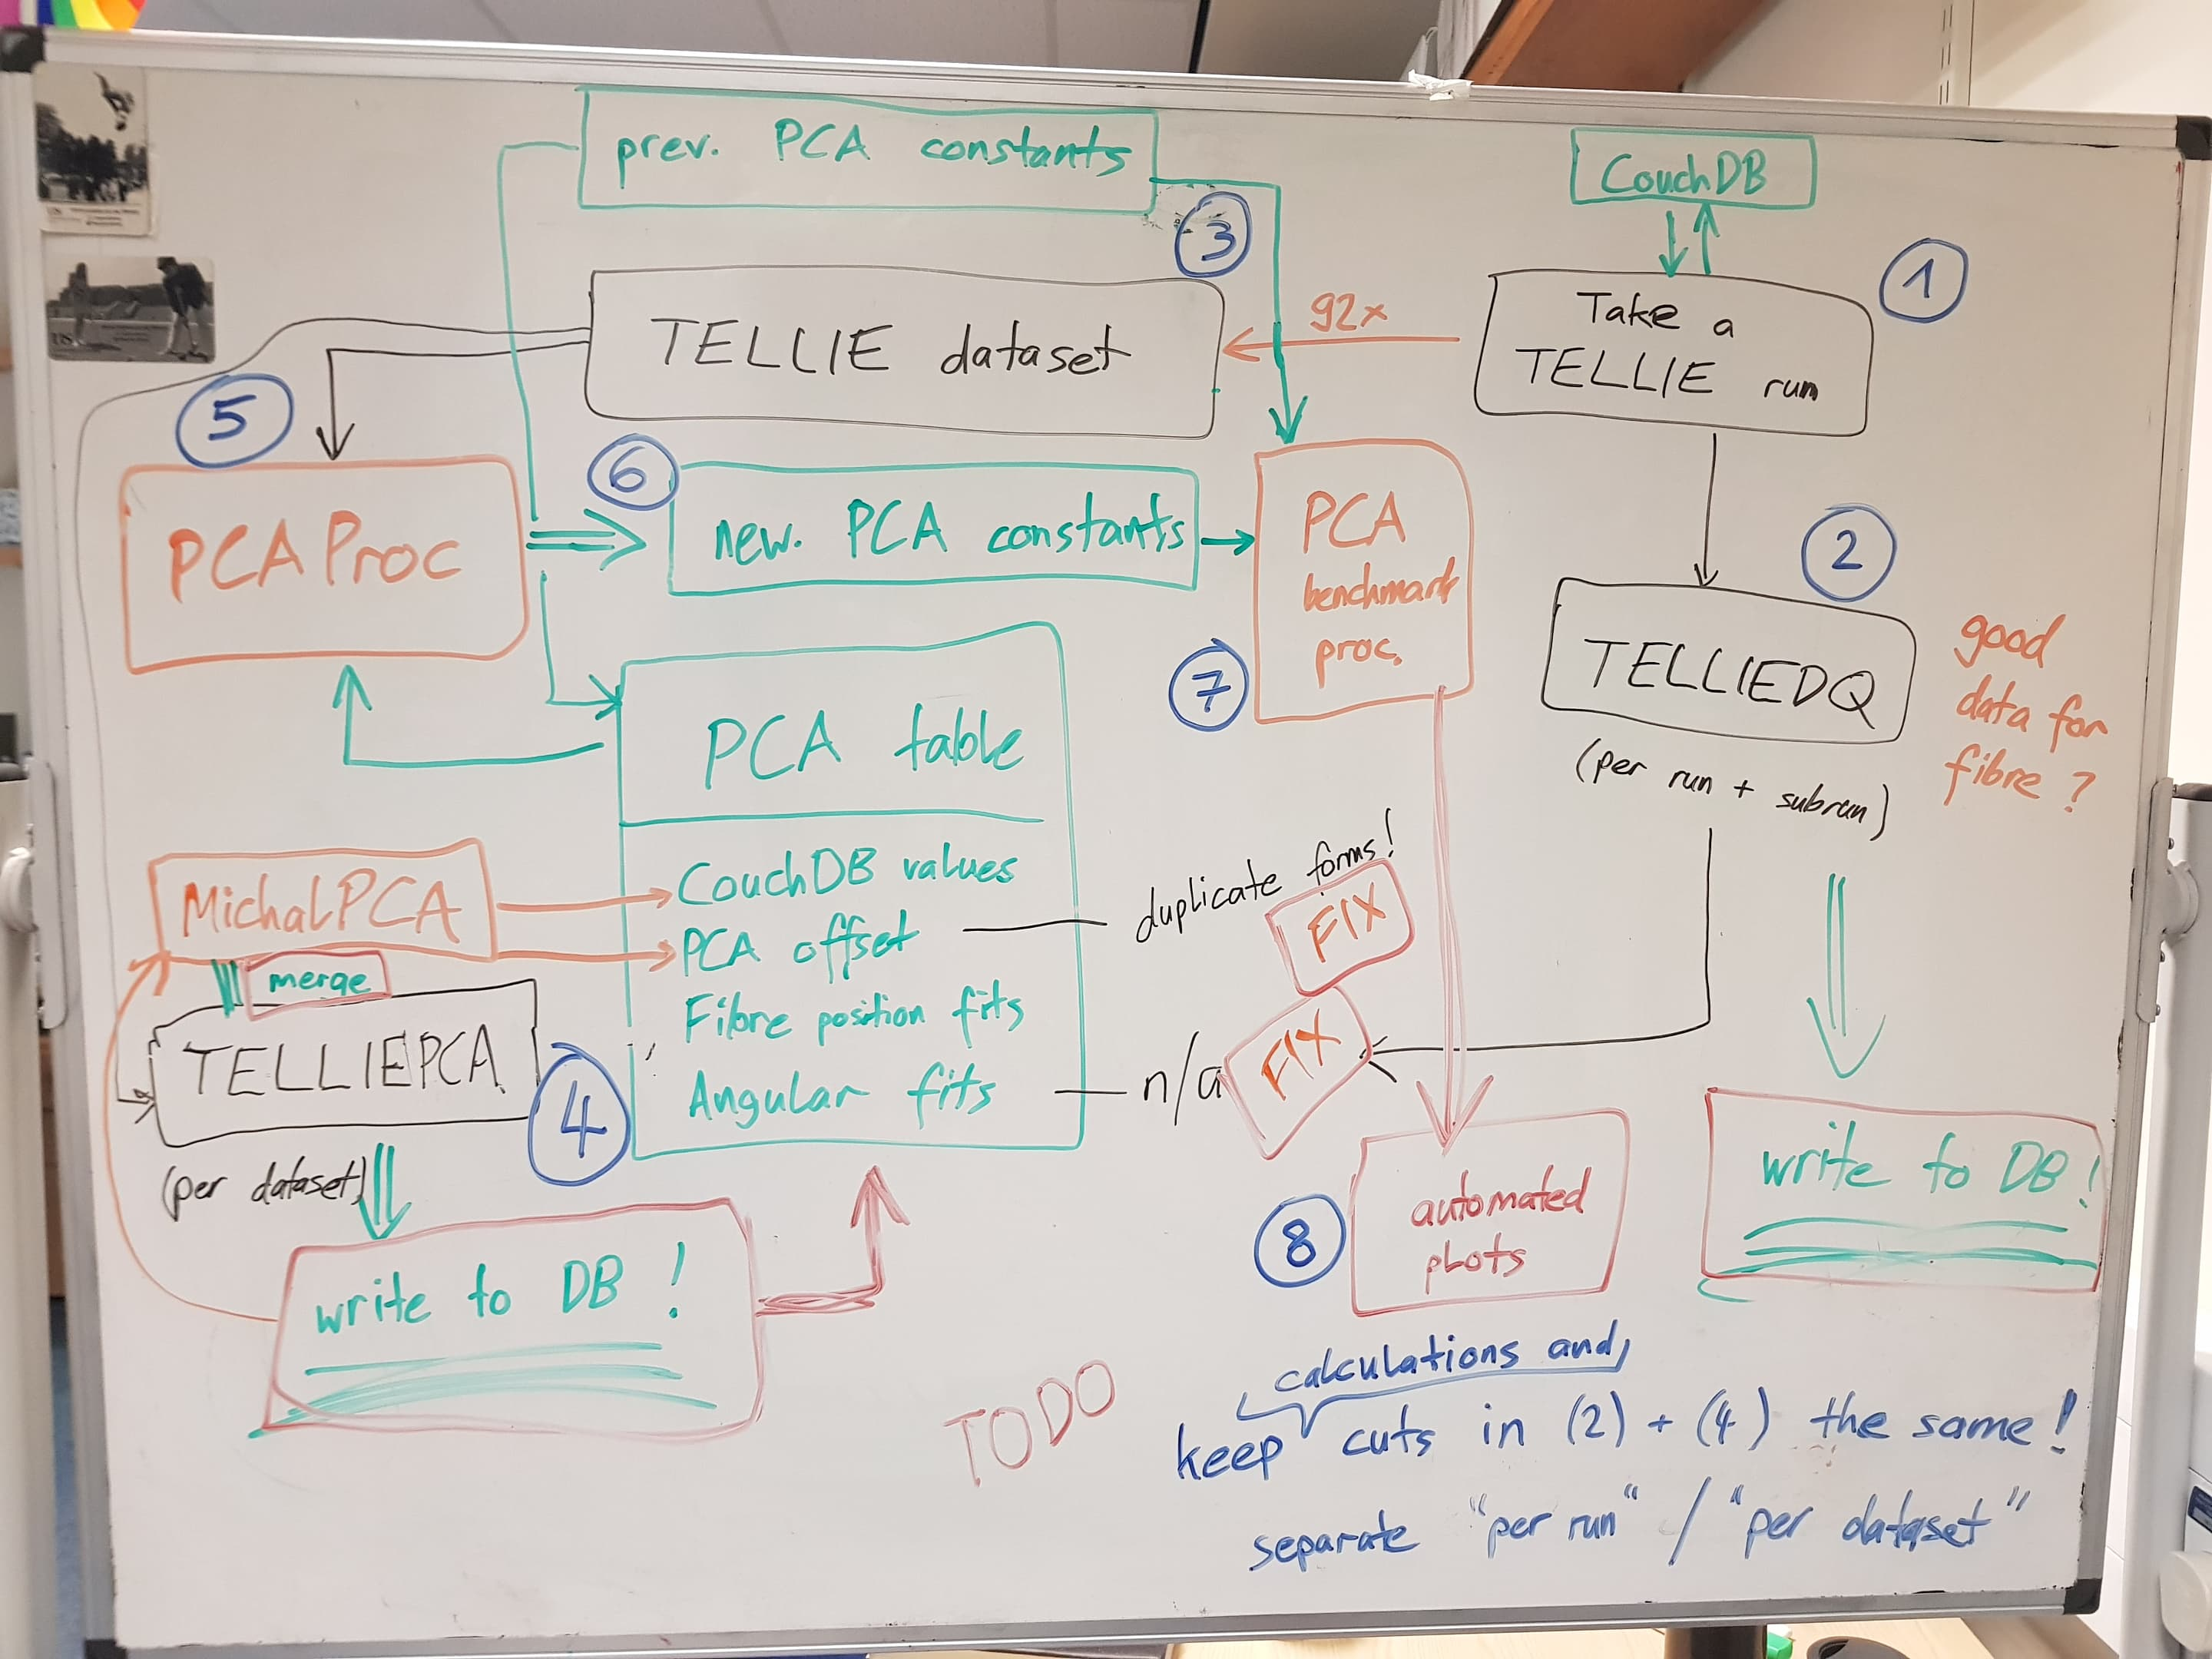
\includegraphics[width=0.9\textwidth]{plots/tellie.jpg}}
\end{frame}

\begin{frame}{Automation: processing}
\begin{itemize}
	\item complex
	\item all the required bits are available
	\item need to unify settings and cuts
	\item needs database interface
	\item need monitoring
\end{itemize}
\end{frame}

\begin{frame}{Automation: what was done}
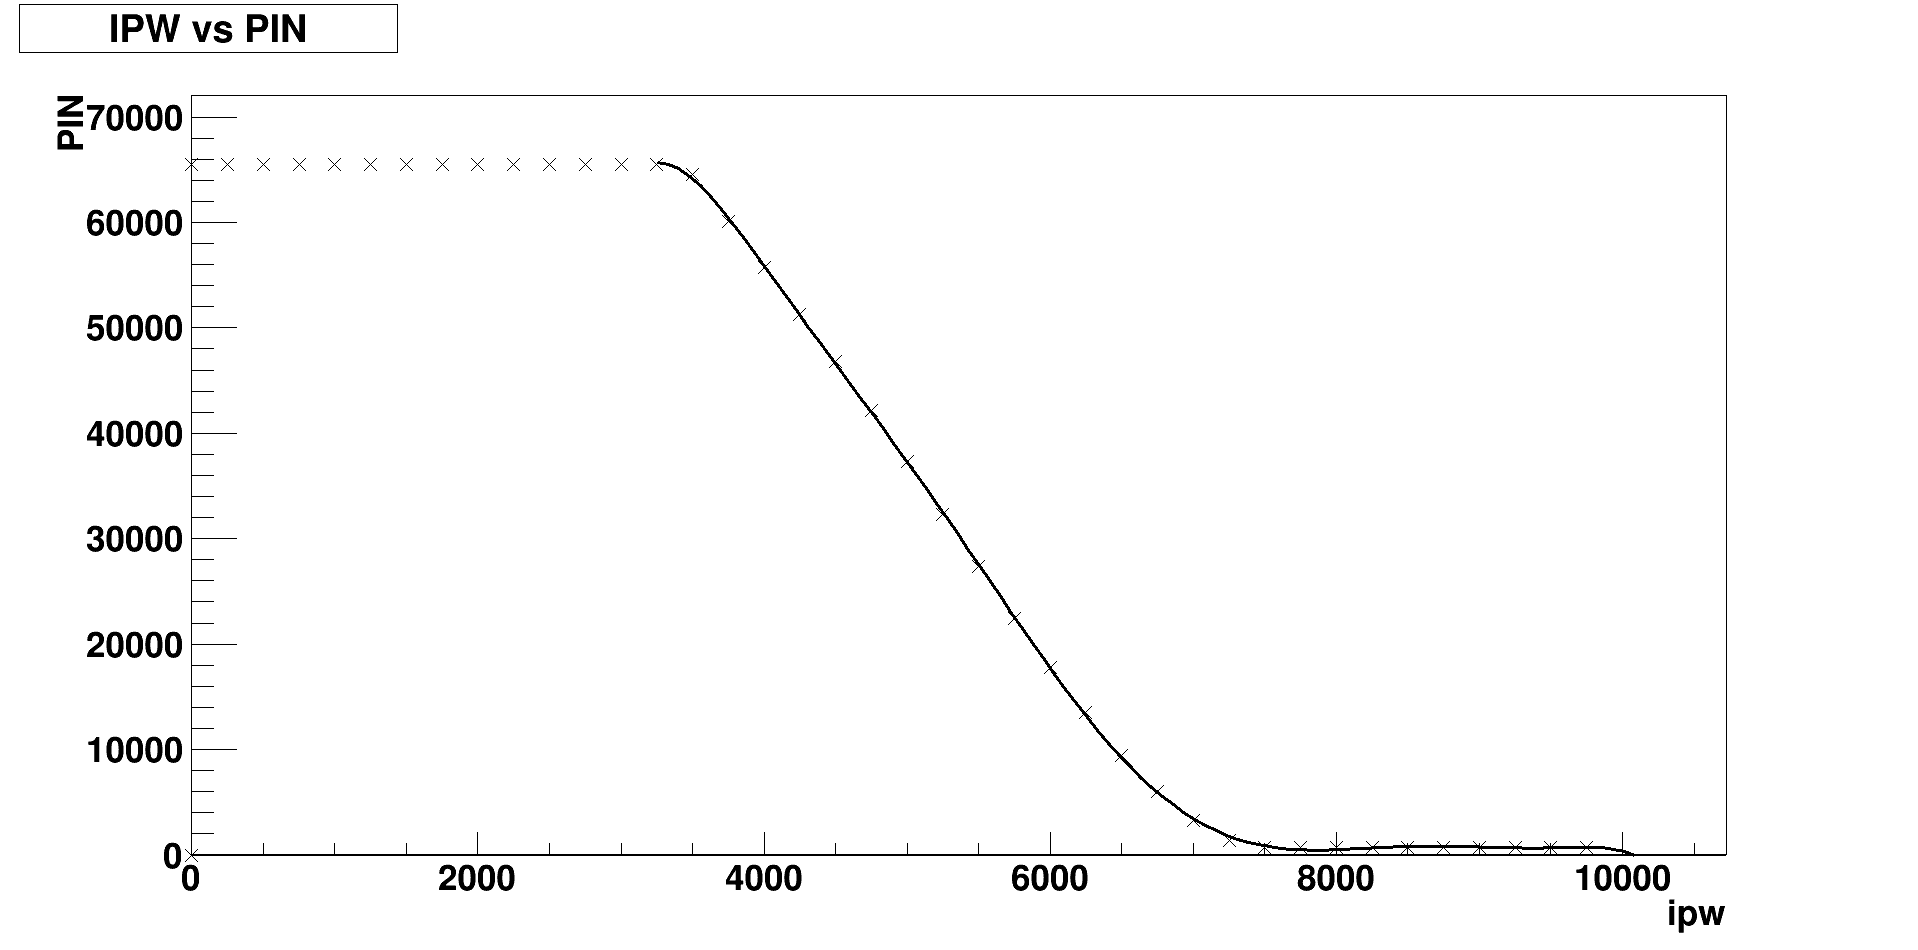
\includegraphics[width=0.49\textwidth]{plots/fit.png}
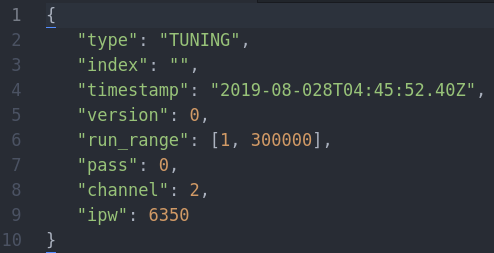
\includegraphics[width=0.49\textwidth]{plots/table.png}
\begin{itemize}
	\item a start was made using teststand and fake tellie server
	\item the calibration curves script written
	\item polynomial fit to PIN response
	\item data upload to database
	\item really just a baby step...
\end{itemize}
\end{frame}

\end{document}